\documentclass[tikz,border=6pt]{standalone}
\usepackage{amsmath}
\usetikzlibrary{arrows.meta,positioning,calc}

\tikzset{
  block/.style={
    draw,
    rectangle,
    minimum width=28mm,
    minimum height=11mm,
    align=center
  },
  sum/.style={
    draw,
    circle,
    minimum size=7mm,
    inner sep=0pt
  },
  line/.style={
    -{Latex[length=2.2mm]},
    thick
  }
}

\begin{document}
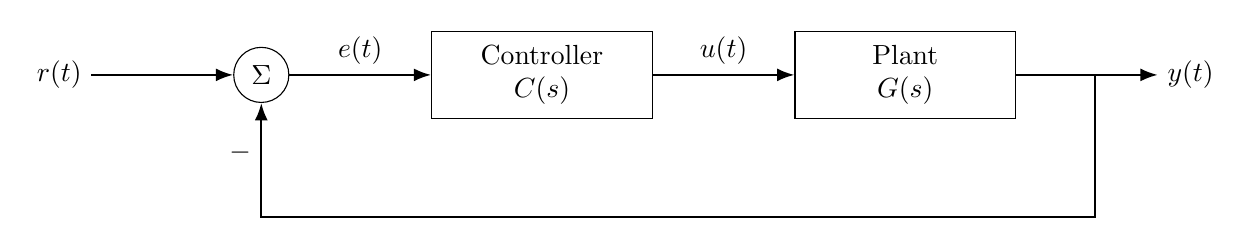
\begin{tikzpicture}[node distance=16mm and 18mm]

\node (r) {$r(t)$};
\node[sum, right=of r] (sum) {$\Sigma$};
\node[block, right=of sum] (controller) {Controller\\$C(s)$};
\node[block, right=of controller] (plant) {Plant\\$G(s)$};
\node[right=of plant] (y) {$y(t)$};

\draw[line] (r) -- (sum);
\draw[line] (sum) -- node[above] {$e(t)$} (controller);
\draw[line] (controller) -- node[above] {$u(t)$} (plant);
\draw[line] (plant) -- (y);

\draw[line] (plant.east) -- ++(10mm,0)
  |- ++(0,-18mm)
  -| node[pos=0.78,left] {$-$} (sum.south);

\end{tikzpicture}
\end{document}
